\setcounter{equation}{0}
\section{Линейные однородные уравнения в частных производных}
\subsection{Основные понятия}
Пусть $\Omega \subset \mathbb R^n$ открыто, $a \in C^1(\Omega, \mathbb R^n)$.
Рассмотрим уравнение
\begin{equation}
    a_1(x)\frac{\partial u}{\partial x_1}(x) + \dots + a_n(x)\frac{\partial u}{\partial x_n}(x) = 0.
\end{equation}
Его решением является функция $u \in C^1(D, \mathbb R)$, где $D \subset \Omega$ открыто, при подстановке которой получается тождественный ноль.
В сокращённой записи:
\[
    \left<a(x), \frac{\partial u}{\partial x}(x)\right> \equiv 0.
\]

\textbf{Определение.} Такое уравнение называется \textit{линейным однородным уравнением в частных производных первого порядка}.

\textbf{Определение.} Система
\begin{equation}
    x' = a(x)
\end{equation}
называется \textit{характеристической системой} уравнения.

Найдём связь между решениями уравнения (1) и его характеристической системы (2).

\textbf{Предложение.} Функция $u \colon D \to \mathbb{R}$ является решением уравнения $(1) \Leftrightarrow u \colon D \to \mathbb{R}$ является первым интегралом системы $(2)$. 

\textbf{Доказательство.} Пусть $u(\cdot)$ --- первый интеграл (2) $\Leftrightarrow$ $\left<a(x), \frac{\partial u}{\partial x}(x) \right> \equiv 0$ по критерию первого интеграла $\Leftrightarrow$ $u(\cdot)$ --- решение уравнения (1).

\QED

Поскольку мы свели задачу к первым интегралам, то для решений уравнения (1) выполняются все те же свойства, что и для первых интегралов (доказываются тривиально).

\textbf{Предложение.} Пусть $u_1, \dots, u_k\colon D \to \mathbb{R}$ --- решения уравнения (1), $(u_1(x), \dots, u_k(x)) \in Y$ для всех $x \in D$, где $Y$ открыто. Тогда для любой функции $F \in C^1(Y, \mathbb{R})$ функция
$u(x) \coloneq F(u_1(x), \dots, u_k(x))$ тоже является решением уравнения (1).

\textbf{Предложение} Пусть $x_0 \in \Omega: a(x_0) \neq 0$. Тогда существуют окрестность $X(x_0)$ и $n-1$ функционально независимых решений $u_1, \dots, u_{n-1} \colon X(x_0) \to \mathbb{R}$ уравнения $(1)$. 

\textbf{Предложение.} Пусть $x_0 \in \Omega: a(x_0) \ne 0$, $D \subset \Omega$ открыто, $u_1, \dots, u_{n-1}\colon D \to \mathbb R$ --- функционально независимые решения уравнения (1).
Тогда существуют окрестности $X(x_0)$ и $Y((u_1(x_0), \dots, u_{n-1}(x_0)))$ такие, что для любого решения $u\colon X(x_0) \to \mathbb R$ уравнения (1) существует функция $F \in C^1(Y, \mathbb{R}) : u(x) \equiv F(u_1(x), \dots, u_{n-1}(x))$.

\subsection{Задача Коши для ЛДУ в частных производных}

Пусть заданы гладкие функции $g, \phi \colon \Omega \to \mathbb R$, причём $\frac{\partial g}{\partial x}(x) \ne 0$ на $\Omega$.
Зададим множество $\gamma := \{x: g(x) = 0\}$ и будем предполагать, что оно непусто, более того, это $(n-1)$--мерная поверхность.
Рассмотрим задачу Коши
\begin{equation}
    \begin{cases}
        \left<a(x), \frac{\partial u}{\partial x}(x) \right> = 0 \\
        u(x) = \phi(x) \text{ при $x \in \gamma$}
    \end{cases}.
\end{equation}

В задаче Коши для ОДУ мы искали решение, которое только в одной точке удовлетворяло начальному условию.
Здесь же мы ищем решение уравнения в частных производных, которое на поверхности $\gamma$ совпадает с заданной функцией $\phi(x)$.

\textbf{Определение.} Функция $\phi$ называется \textit{начальным значением} функции $u$ на $\gamma$.

\textbf{Определение.} Поверхность $\gamma$ называется \textit{начальной поверхностью}.

\textbf{Определение.} Точка $\widehat{x} \in \Omega$ называется \textit{характеристической точкой} задачи (3), если $\widehat{x} \in \gamma$ и $\left<a(\widehat{x}), \frac{\partial g}{\partial x}(\widehat{x}) \right> = 0$.

\begin{figure}[h]
    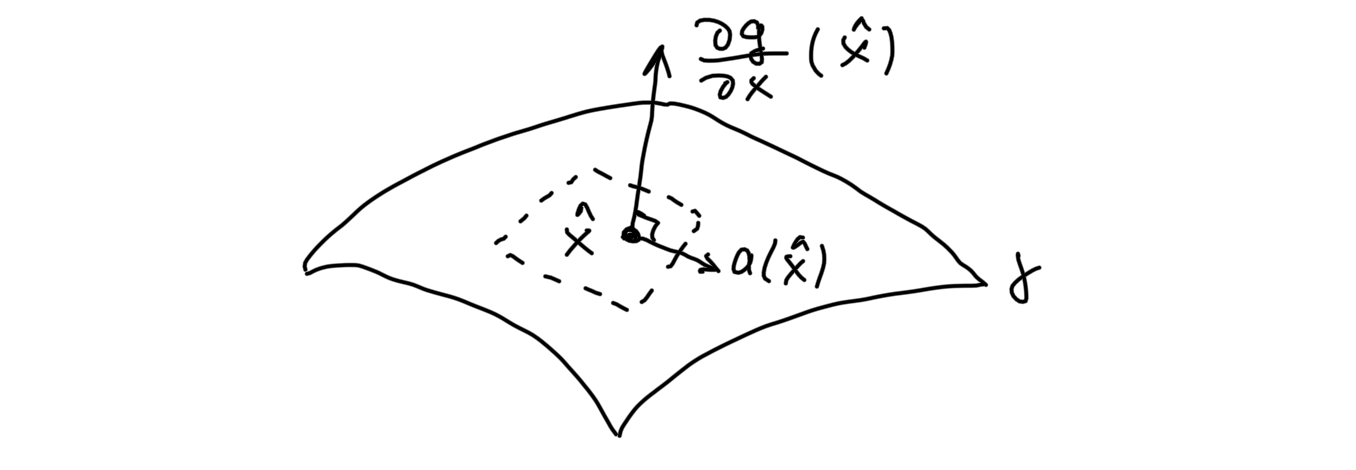
\includegraphics[scale=0.4]{characteristic-point}
    \centering
    \caption{Визуализация характеристической точки}
\end{figure}

\textbf{Теорема.} Пусть точка $\widehat{x} \in \gamma$ не является характеристической.
Тогда существуют окрестность $V(\widehat x)$ и функция $u\colon V(\widehat{x}) \to \mathbb R$ такая, что она является единственным решением задачи (3) в этой окрестности.

\textbf{Доказательство.} Мы знаем, что $a(\widehat{x}) \ne 0$. Тогда можно применить одно из предложений выше: существуют окрестность $X(\widehat{x})$ и функции $u_2, \dots, u_n \colon X(\widehat{x}) \to \mathbb{R}$ такие, что 
$u_2, \dots, u_n$ -- функционально независимые решения задачи (1). 

Зададим отображение $\Phi\colon X(\widehat{x}) \to \mathbb{R}^n$ следующим образом:
$$
\Phi(x) \coloneq 
\begin{pmatrix}
    g(x)\\
     u_2(x)\\
     \vdots\\
     u_n(x)\\
\end{pmatrix}.
$$
Хотим применить теорему об обратной функции, проверим, что матрица Якоби
\[ 
    \begin{pmatrix}
        \frac{\partial g}{\partial x}(\widehat{x}) \\[5pt]
        \frac{\partial u_{2}}{\partial x}(\widehat{x}) \\
        \vdots \\
        \frac{\partial u_{n}}{\partial x}(\widehat{x})
    \end{pmatrix}
\]
невырождена. Докажем от противного: пусть
\[
    \frac{\partial g}{\partial x}(\widehat x) = \sum_{j=2}^{n} \lambda_j \frac{\partial u_j}{\partial x}(\widehat x).
\]
Это рассматривать достаточно, так как первые $n - 1$ строк точно линейно независимы.
Умножим скалярно на $a(\widehat x)$:
\[
    \left< a(\widehat x), \frac{\partial g}{\partial x}(\widehat x) \right> = \sum_{j=2}^{n} \lambda_j \left< a(\widehat x), \frac{\partial u_j}{\partial x}(\widehat x) \right> = 0,
\]
так как $u_j$ --- решения уравнения (1).
Противоречие с тем, что $\widehat x$ не является характеристической точкой. 

Теперь по теореме об обратном отображении найдутся окрестности $V(\widehat x) \subset X(\widehat{x})$,\\
$W((u_2(\widehat x), \dots, u_{n}(\widehat x))) \subset \mathbb{R}^{n-1}$ и $\varepsilon > 0$ такие, что $\Phi \colon V \to (-\varepsilon, \varepsilon) \times W$ является диффеоморфизмом. Построим решение задачи Коши. Возьмём функцию $$u(x) \coloneq \phi(\Phi^{-1}(0, u_2(x), \dots, u_n(x)))$$
для всех $x \in V(\widehat{x})$. Заметим, что $u$ -- решение уравнения (1). Покажем, что $u$ также является решением задачи Коши. Берём $x \in \gamma \Rightarrow g(x) = 0$:
$$u(x) = \phi(\Phi^{-1}(0, u_2(x), \dots, u_n(x))) = \phi(\Phi^{-1}(g(x), u_2(x), \dots, u_n(x))) = \phi(\Phi^{-1}(\Phi(x))) = \phi(x).$$
Таким образом, мы доказали существование решения. Докажем теперь единственность.

Для этого уменьшим окрестности $V$, $W$ и $\varepsilon$ так, чтобы для любого решения $v \colon V \to \mathbb{R}$ уравнения (1) существовала функция $F \in C^1(W, \mathbb{R}) : v(x) \equiv F(u_2(x), \dots, u_n(x))$.
Возьмём на меньшей окрестности решение $v \colon V \to \mathbb{R}$ задачи Коши (3) и покажем, что оно совпадает с уже найденным решением $u$.

Во-первых, для него выполняется $v(x) \equiv F(u_2(x), \dots u_n(x))$. Возьмём $x \in \gamma \Rightarrow v(x) = \phi(x) = u(x)$, так как и $u, v$ являются решениями задачи Коши. Значит, $F(u_2(x), \dots u_n(x)) \equiv \phi(\Phi^{-1}(0, u_2(x), \dots, u_n(x)))$.
Поскольку $\Phi$ --- это диффеоморфизм, то для любой точки\\$(y_1, \dots, y_n) \in W$ верно: $F(y_2, \dots, y_n) \equiv \phi(\Phi^{-1}(0, y_2, \dots, y_n)).$
Тогда $$v(x) \equiv F(u_2(x), \dots, u_n(x)) \equiv \phi(\Phi^{-1}(0, u_2(x), \dots, u_n(x))) \equiv u(x).$$

\QED

\textbf{Пример.} Рассмотрим уравнение $u_x + u_y = 0$ и начальное условие
$$
\begin{cases}
  u(x, y) = 1\\
  x-y = 0
\end{cases}.
$$
Перейдем к характеристической системе 
$$
 \begin{cases}
    x' = 1\\
    y' = 1
 \end{cases}.
$$
Тогда $x - y = C$ --- это первый интеграл. Рассмотрим произвольную функцию $F$: $F(0) = 1$.
Отсюда $u(x, y) = F(x-y)$ является решением задачи Коши, то есть решений бесконечно много.

Рассмотрим теперь то же уравнение, но с другим начальным условием:
$$
\begin{cases}
   u(x, y) = x^2+y^2\\
   x-y = 0
\end{cases}.
$$

Знаем, что $u(x, y) = F(x-y)$ --- это общее решение. При $x-y = 0$ получаем $u(x, y) = F(0)$. Значит, для всех решений задачи Коши $F(0) = x^2+y^2$ на прямой $x-y = 0$. Такого быть не может, потому что $F(0)$ --- константа. То есть у этой задачи Коши нет решений. 

В этих примерах не выполняется условие теоремы, потому что все точки на кривой $\gamma$ являются характеристическими.

Действительно,
$$
a =
\begin{pmatrix}
1\\
1
\end{pmatrix},\;\;
\frac{\partial g}{\partial x} =
\begin{pmatrix}
1\\
-1
\end{pmatrix},
$$
а их скалярное произведение равно нулю во всех точках.